\documentclass[../../index.tex]{subfiles}

\begin{document}
\chapter{$\tau$ decays into hadrons}
The $\tau$-lepton is the only lepton heavy enough to decay into Hadrons. It
permits one of the most precise determinations of the strong coupling $\alpha_s$.
The inclusive $\tau$-decay ratio
\begin{equation}
  \label{eq:inclusiveRatio}
  R_\tau = \frac{\Gamma(\tau \to \nu_\tau + \text{Hadrons})}{\Gamma(\tau \to \nu_\tau e^+ e^-)}
\end{equation}
can be precisly calculated and is sensitive to $\alpha_s$. Due to low the mass of
the $\tau$-lepton $m_\tau\approx\SI{1.8}{\giga\eV}$ $\tau$-decays are excellent
for performing a low-energy QCD analysis.
The theoretical expression of the hadronic $\tau$-decay ratio was first derived
by \cite{Tsai1971}, using current algebra, a more recent derivation making use
of the \textit{optical theorem} can be taken from \cite{Schwab2002}. The
inclusive ratio is then given by:
\begin{equation}
  \label{eq:hadronicTauDecayRatio}
  R_\tau(s) = 12 \pi \int_0^{m_\tau} = \frac{\dif s}{m_\tau^2}
  \left( 1 - \frac{s}{m_\tau^2} \right)
  \left[ \left( 1 + 2 \frac{s}{m_\tau^2} \right) \Ima \Pi^{(T)}(s) + \Ima \Pi^{(L)}(s) \right],
\end{equation}
where $\Ima \Pi$ is the two-point function (see \cref{sec:twoPointFunction}). In
the case of $\tau$-decays we only have to consider vector (V) and axial-vector
contributions (A) of decays into up, down and strange quarks. Thus taking $i,j$ as the flavour
indices for the light quarks (u, d and s) we can express the correlator as
\begin{equation}
  \Pi_{\mu\nu,ij}^{V/A}(s) \equiv i \int \dif x \,e^{ipx} \langle \Omega | T \{ J_{\mu,ij}^{V/A}(x) J_{\nu,ij}^{V/A}(0)^\dagger \} | \Omega \rangle,
\end{equation}
with $|\Omega\rangle$ being the physical vacuum. The vector and axial-vector
currents are then distinguished by the corresponding dirac-matrices
($\gamma_\mu \text{and} \gamma_\mu \gamma_5$) given by
\begin{equation}
  J_{\mu,ij}^{V}(x) = \anti{q}_j(x) \gamma_\mu q_i(x) \quad \text{and} \quad J_{\mu,ij}^{A}(x) = \anti{q}_j(x) \gamma_\mu \gamma_5 q_i(x).
\end{equation}
The two-point function can be decomposed into its vector and axial-vector
contributions, but also into transversal and longitudinal components. We will
give now both of these decompositions and relate them, which has some
implications for a common used approximation: the \textbf{chiral limit}, where
the quark masses are taken to 0 ($m_q \to 0$).

Starting with the decomposition into vector, axial-vector, scalar (S) and pseudo-scalar (P) components we can
write \cite{Broadhurst1981,Jamin1992}
\begin{equation}
  \label{eq:correlatorVectorScalarDecomposition}
  \begin{split}
    \Pi^{\mu\nu}(q^2) &= (q^\mu q^\nu - q^2 g^{\mu\nu}) \Pi^{V,A}(q^2) + \frac{g^{\mu\nu}}{q^2} (m_i \mp m_j)\Pi^{S,P}(q^2) \\
    &+ g^{\mu\nu}\frac{(m_i \mp m_j)}{q^2} [ \langle \anti{q}_i q_i \rangle \mp \langle \anti{q}_j q_j \rangle],
  \end{split}
\end{equation}
which is composed of a vector $\Pi^{V,A}$ and scalar $\Pi^{S,P}$ part. The third
term are corrections arising due to the physical vacuum $|\Omega\rangle$. The
latter decomposition rewrites the correlator $\Pi^{\mu\nu}(q^2)$ into transversal
and longitudinal components:
\begin{equation}
  \label{eq:correlatorTransversalLongitudinalDecomposition}
  \Pi^{\mu\nu}(q^2) = (q^\mu q^\nu - g^{\mu\nu}q^2) \Pi^{(T)}(q^2) + q^\mu q^\nu \Pi^{(L)}(q^2).
\end{equation}
With the two decompositions \cref{eq:correlatorVectorScalarDecomposition} and
\cref{eq:correlatorTransversalLongitudinalDecomposition} we can now identify the
longitudinal components of the correlator as being purely scalar, by multiplying
\cref{eq:correlatorVectorScalarDecomposition} by two four-momenta and making use
of the Ward-idendity \cref{eq:wardIdentity} we can write
\begin{equation}
  q_\mu q_\nu \Pi^{\mu\nu}(q^2) = (m_i \mp m_j)^2 \Pi^{S,P}(q^2) + (m_i \mp m_j)[\langle \anti{q}_i q_i \rangle \mp \langle \anti{q}_j q_j \rangle],
\end{equation}
which then can be related to the longitudinal component of
\cref{eq:correlatorTransversalLongitudinalDecomposition} by comparisson of the
two equations
\begin{equation}
  q_\mu q_\nu \Pi^{\mu\nu}(q^2) = q^4 \Pi^{(L)}(q^2) = s^2 \Pi^{(L)}(s) \quad \text{with} \quad s\equiv q^2.
\end{equation}
In a more eloquent way this can be expressed as
\begin{equation}
  s^2 \Pi^{(L)}(s) = (m_i \mp m_j)^2 \Pi^{(S,P)}(s) + (m_i \mp m_j)[ \langle \anti{q}_i q_i \rangle \mp \langle \anti{q}_j q_j \rangle],
\end{equation}
where we can see, that all mass terms are related to the longitudinal component
of the correlator. By defining a combination of the transversal and longitudinal
correlator
\begin{equation}
  \label{eq:correlatorCombination}
  \Pi^{(T+L)}(s) \equiv \Pi^{(T)}(s) + \Pi^{(L)}(s)
\end{equation}
we can additionaly relate the transversal and vectorial components via
\begin{equation}
  \label{eq:longitudinalCorrelator}
  \begin{split}
    \Pi^{\mu\nu}(s) &= \underbrace{(q^\mu q^\nu - g^{\mu\nu}q^2)\Pi^{(T)}(s) + (q^\mu q^\nu - g^{\mu\nu} q^2)\Pi^{(L)}(s)}_{=(q^\mu q^\nu - g^{\mu\nu} q^2) \Pi^{(T+L)}(s)} + \frac{g^{\mu\nu}s^2}{q^2}\Pi^{(L)}(s),
  \end{split} 
\end{equation}
such that
\begin{equation}
  \Pi^{(V,A)}(s) = \Pi^{(T)}(s) + \Pi^{(L)} = \Pi^{(T+L)},
\end{equation}
where the vector/ axial-vector component of the correlator is now related to the
newly defined transversal and longitudinal combination of the correlator. As the
$\tau$-decays, with the limiting factor of the $\tau$-mass, can only decay into
light quarks we will often neglect the quark masses and work in the so called
chiral limit. In the chiral limit the longitudinal component, which is 
proportional to the quark masses, of the correlator vanishes.  

Examining the inclusive ratio $R_\tau$ in \cref{eq:inclusiveRatio}, we note that
we have to deal with a problematic integral over the real axis of $\Pi(s)$ from
$0$ up to $m_\tau$. The integral is problematic for two reasons:
\begin{itemize}
  \item \textbf{Perturbative Quantum Chromodynamcs} (pQCD) and the OPE breaks down for low
    energies (over which we have to integrate).
  \item The positive euclidean axis of $\Pi(s)$ has a discontinuity cut and can
    theoretically not be evaluated (see \cref{sec:twoPointFunction}).
\end{itemize}
To literally circunvent the former issue we make use of \textit{Cauchy's Theorem}
\cref{eq:cauchysTheorem}. For the latter we will apply so-called \textbf{pinched weights}.

\section{Rescuing pQCD with Cauchy's theorem}
We will make use of Cauchy's theorem to rewrite the definite integral of
\cref{eq:hadronicTauDecayRatio} into a contour integral over a closed circle
with radius $m_\tau^2$. The closed contour consists of four line integrals,
which have been visualized in \cref{fig:rTauCauchysTheorem}. Summing over the
four line integrals, performing a \textit{analytic continuation} of the
two-point correlator $\Pi(s) \to \Pi(s + i \epsilon)$ and finally taking the
limit of $\epsilon \to 0$ gives us the needed relation between
\cref{eq:hadronicTauDecayRatio} and the closed contour:
\begin{equation}
  \begin{split}
  \oint_{s=m_\tau} \Pi(s) &= \int_0^{m_\tau} \Pi(s + i \epsilon) + \int_{\mathcal{C}_2}\Pi(s) \dif s + \int_{m_\tau}^0 \Pi(s - i \epsilon) \dif s + \int_{\mathcal{C}_4} \Pi(s) \dif s \\
  &= \int_0^{m_\tau} \Pi(s+i \epsilon) - \Pi(s - i \epsilon) \dif s  + \int_{\mathcal{C}_2}\Pi(s) \dif s + \int_{\mathcal{C}_4} \Pi(s) \dif s \\
  &= \int_0^{m_\tau} \Pi(s + i \epsilon) - \overline{\Pi(s + i \epsilon)} + \int_{\mathcal{C}_2}\Pi(s) \dif s + \int_{\mathcal{C}_4} \Pi(s) \dif s \\
  &\overset{\lim \epsilon \to 0}{=} 2 i \int_0^{m_\tau} \Ima \Pi(s) \dif s + \oint_{s=m_\tau} \Pi(s) \dif s
  \end{split}
\end{equation}
where we made use of $\Pi(z) = \overline{\Pi(\overline z)}$ (due to $\Pi(s)$ is analytic) and
$\Pi(z) - \overline{\Pi(z)} = 2 i \Ima \Pi(z)$. The result can be rewritten in a
more intuitive form, which we also visualized in \cref{fig:rTauCauchysTheorem}
\begin{equation}
  \label{eq:correlatorContourIntegral}
  \int_0^{m_\tau} \Pi(s) \dif s = \frac{i}{2} \oint_{s=m_\tau} \Pi(s) \dif s
\end{equation}
\begin{figure}
  \centering
  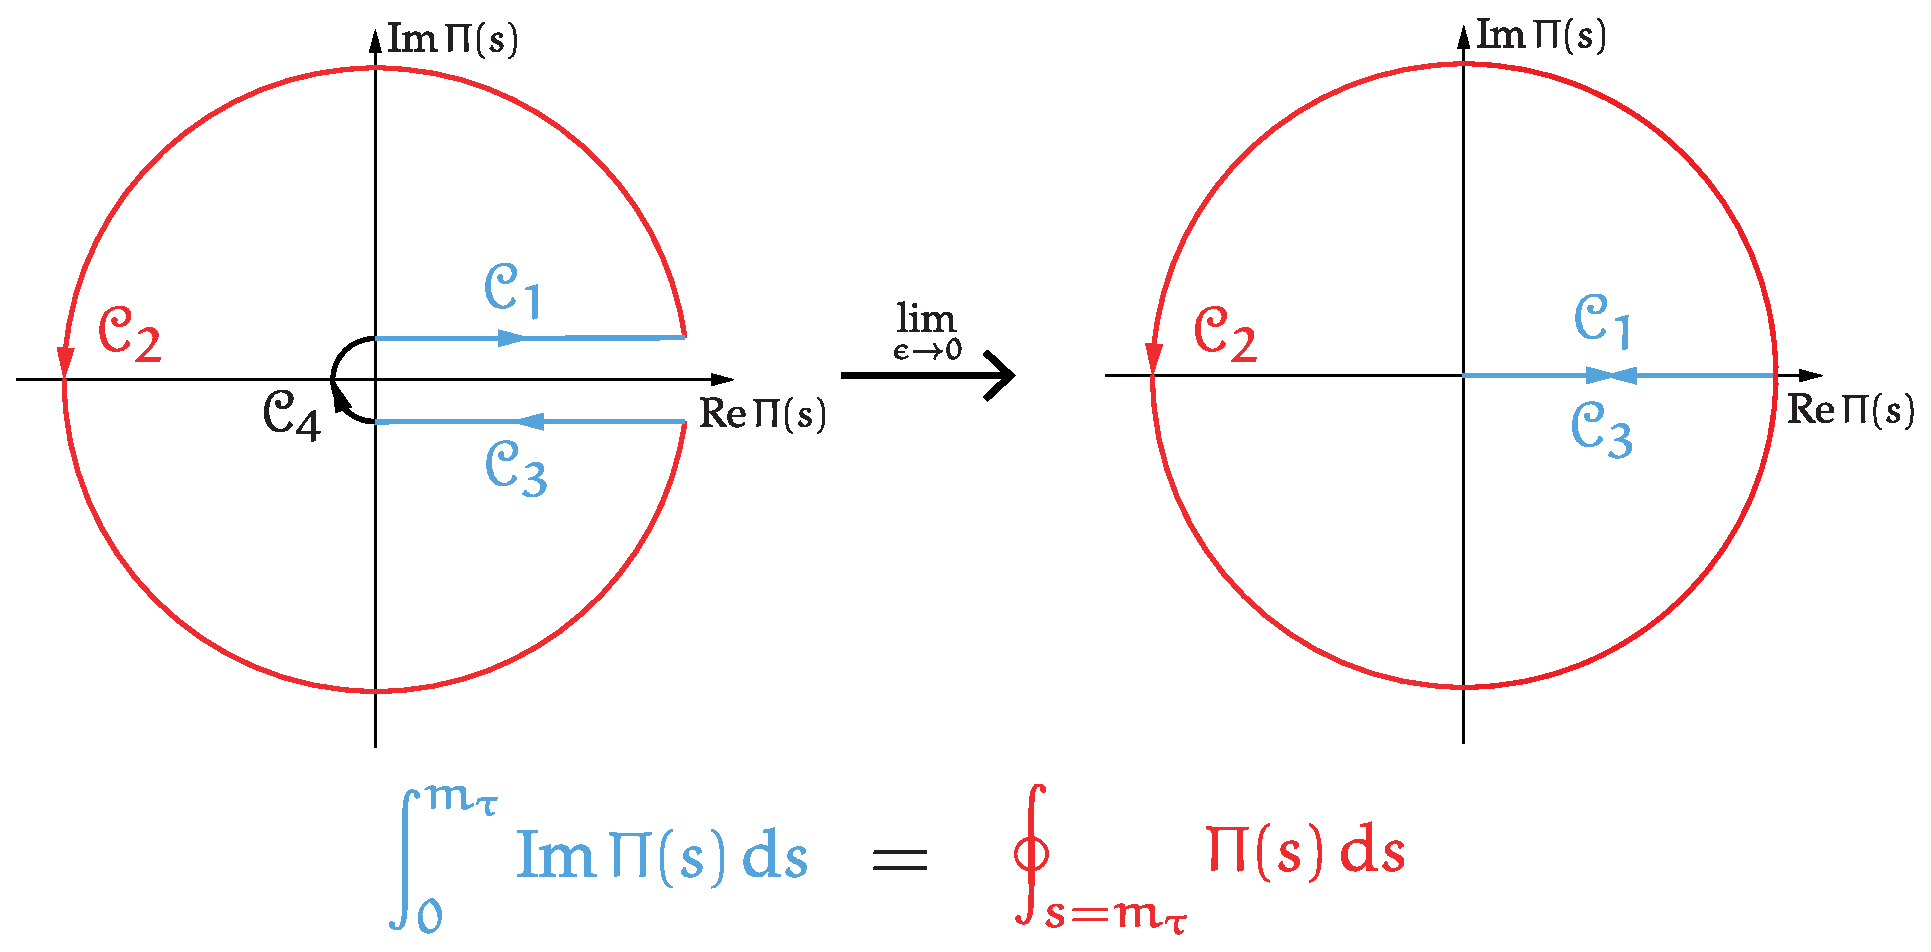
\includegraphics[width=0.8\textwidth]{./images/rTauCauchysTheorem.eps}
  \caption{Visualization of the usage of Cauchy's theorem to transform
    \cref{eq:hadronicTauDecayRatio} into a closed contour integral over a circle
  of radius $m_\tau^2$.}
  \label{fig:rTauCauchysTheorem}
\end{figure}
Due to the circle-contour we can avoid low energies at
which pQCD would break down. 

To deal with the latter issue we have to suppress the contributions of the
correlator close to the positive real axis, which can be achieved by introducing
weight functions, which suppress contributions of the two-point function close
to the postive real axis.

Finally combining \cref{eq:correlatorContourIntegral} with
\cref{eq:hadronicTauDecayRatio} we get
\begin{equation}
  \label{eq:rTauT+L}
  R_\tau = 6 \pi i \oint_{s=m_\tau} \frac{\dif s}{m_\tau^2}
  \left( 1 - \frac{s}{m_\tau^2} \right)
  \left[ \left( 1 + 2 \frac{s}{m_\tau^2} \right) \Pi^{(T)}(s) + \Pi^{(L)} \right]
\end{equation}
for the hadronic $\tau$-decay ratio. It is convenient to work with
$\Pi^{(T+L)}$, which is connected to the vector/ axial-vector components of the
correlator. Thus using \cref{eq:correlatorCombination} in \cref{eq:rTauT+L} yields
\begin{equation}
  R_\tau = 6 \pi i \oint_{\abs{s}=m_\tau} \frac{\dif s}{m_\tau^2} \left( 1 - \frac{s}{m_\tau^2} \right)^2 \left[ \left( 1 + 2 \frac{s}{m_\tau^2} \right) \Pi^{(L+T)}(s) - \left( \frac{2 s}{m_\tau^2} \right) \Pi^{(L)}(s) \right]
\end{equation}

By introducing Cauchy's theorem we avoided low energies, which could lead to a
breakdown of PT. The contour integral obtained is an important result as we are
now able to theoretically evaluate the hadronic $\tau$-decay ratio at
sufficiently large energy scales ($m_\tau \approx \SI{1.78}{\mega\eV}$)
at which $\alpha_s(m_\tau)\approx 0.33$ \cite{Pich2016} is large enough to
apply perturbation theory and the OPE. Obviously we would benefit from a
contour integral over a bigger circunference, but $\tau$-decays are limited by the $m_\tau$.
Nevertheless there are promising $e^+e^-$ annihilation data, which yields
valuable R-ratio values up to $\SI{2}{\giga\electronvolt}$
\cite{Boito2018}\cite{Keshavarzi2018}.

\section{Pinched weights to avoid DVs}
We are free to multiply \cref{eq:correlatorContourIntegral} by an analytic weight function $\omega(s)$
\begin{equation}
  \int_0^{m_\tau} \omega(s) \Pi(s) \dif s = \frac{i}{2} \oint_{s=m_\tau} \omega(s) \Pi(s) \dif s.
\end{equation}
We can use this technique to suppress contributions for the two-point function
close to the positive real axis by implementing so called \textbf{pinched
  weights} of the form
\begin{equation}
  \omega(s) = (1-\frac{s}{m_\tau^2})^k,
\end{equation}
where k is the degree of the pinched weight. The heigher the degree the farther
we operate from the critical postivie real axis (see. \cref{fig:pinchedWeightGraphs}), which suppresses the effects of
duality violations. This pinching of second degree appears quite naturally.
\begin{figure}
  \centering
  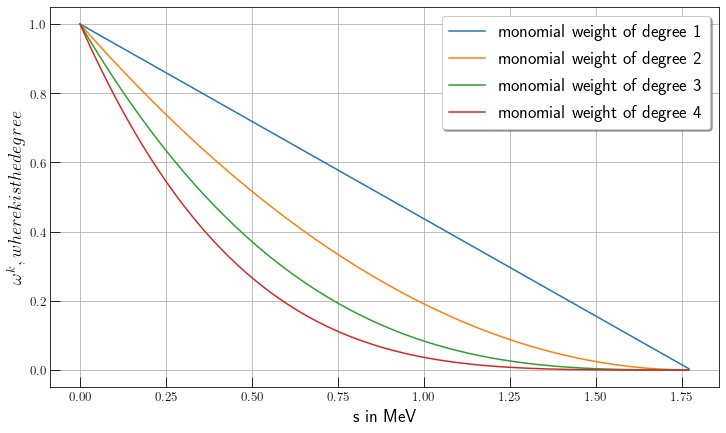
\includegraphics[width=\textwidth]{./images/monomialWeightGraphs.png}
  \caption{Monomial weights $(1-s/m_\tau^2)^k$ for degrees $1\to4$. We can see
    that weights of heigher pinching decrease faster, which comes in handy if we
  want to suppress duality violations.}
  \label{fig:monomialWeightGraphs}
\end{figure}
If we regard the incluse $\tau-decay$ ratio \cref{eq:rTauT+L}, we note that for the
transversal component we already have a double pinched weight, the
\textit{kinematic weight}
\begin{equation}
  \label{eq:kinematicWeight}
  \omega_\tau(s) = \left( 1-\frac{s}{m_\tau^2} \right) \left( 1 + 2 \frac{s}{m_\tau^2} \right).
\end{equation}
In general it is said that a double pinched weight is sufficient to neglect
effects caused by duality violation.

We can also use different weights to control the dimensions of the OPE that
contribute. The weights we are using have to be analytic, so that we can make
use of Cauchy's theorem. Thus they can be represented as polynomials
\begin{equation}
  \omega(x) = \sum_i a_i x^i,
\end{equation}
every contributing monomial is responsible for a dimension of the OPE.
Dimensions that are not represented in the weight polynomial do not contribute
at all or are very suppressed as we will demonstrate now.

The residue of a monomial $x^k$ is only different from 0 if its power $k=-1$:
\begin{equation}
  \label{eq:monomialWeights}
  \oint_{C} x^k \dif x = i \int_0^{2\pi}\left(e^{i \theta}\right)^{k+1} \dif \theta
  = \begin{cases} \mbox{$2 \pi i$} & \mbox{if } k=-1, \\ \mbox{0} & \mbox{otherwise} \end{cases}.
\end{equation}
Consequently if we exchange the kinematic weight of the incluse ratio
\cref{eq:inclusiveRatio} through a monomial and neglect all terms of no interest
to us we can write
\begin{equation}
  \label{eq:monomialInclusiveRatio}
  \begin{split}
  \left. R(x m_\tau) \right\rvert_{D=0,2,4\dots} &= \oint_{\abs{x}=1} \frac{x^k}{(x m_\tau)^{\frac{D}{2}}}C^{D}(x m_\tau) \\
  &= \frac{1}{(m_\tau)^{\frac{D}{2}}} \oint_{\abs{x}=1} x^{k-D/2} \,C^{D}(x m_\tau),
  \end{split}
\end{equation}
where $C^{D}$ are the $D$-dimensional Wilson coefficients. Thus combining
\cref{eq:monomialWeights} with \cref{eq:monomialInclusiveRatio} we see that
only Dimension  which fulfill
\begin{equation}
  k - D/2 = -1 \quad \implies \quad  D = 2(k+1)
\end{equation}
contribute to the OPE. For example the polynomial of the kinematic weight is
given by
\begin{equation}
  (1 - x)^2 (1 + 2x) = \underbrace{1}_{D=2} - 3\underbrace{x^2}_{D=6} + 2\underbrace{x^3}_{D=8},
\end{equation}
where we underbraced the monomials and gave the active dimensions. A list of
monomomials and their corresponding Dimensions up to dimension 14 can be found
in \cref{table:monomialDimensions}.
\begin{table}
  \centering
  \begin{tabular}{l|lllllll}
    \toprule
    \textbf{monomial:} & $x^0$ & $x^1$ & $x^2$ & $x^3$ & $x^5$ & $x^6$ & $x^7$\\
    \textbf{dimension:} & $D^{(2)}$ & $D^{(4)}$ & $D^{(6)}$ & $D^{(8)}$ & $D^{(10)}$ & $D^{(12)}$ & $D^{(14)}$\\
    \bottomrule 
  \end{tabular}
  \caption{List of monomials and their corresponding ``active'' dimensions in the OPE.}
  \label{table:monomialDimensions}
\end{table}
This behaviour enables us to bring out different dimensions of the OPE and
suppress contributions of heigher order ($D\geq10$) for which less is kown. 


\section{RG invariance}
The two-point function is not a physical quantity. It does not fulfill the RGE
\cref{eq:RGE} and is thus dependent on the scale $\mu$. We can enhance the
inclusive ration \cref{eq:inclusiveRatio} making use of the \textbf{Adler function} defined as:
\begin{equation}
  \label{eq:adlerFunction}
  D^{(T+L)}(s) \equiv -s \od{}{s} \Pi^{(T+L)}(s), \qquad D^{(L)}(s) \equiv \frac{s}{m_\tau^2} \od{}{s} (s \Pi^{(L)}(s)),
\end{equation}
where we have two separate definitions: one for the transversal plus longitudinal
contribution and one for solely longitudinal part. The two-point functions can now be replaced with the help of partial integration
\begin{equation}
  \int_a^b u(x) V(x) \dif x = \left[ U(x) V(x) \right]_a^b - \int_a^b U(x) v(x) \dif x.
\end{equation}
We will do the computation for each of the two cases $(T+L)$ and $(L)$ separate.
Starting by the transversal plus longitudinal contribution we get:
\begin{equation}
  \begin{split}
    R_\tau^{(1)} &= \frac{6 \pi i}{m_\tau^2} \oint_{\abs{s}=m_\tau^2}\underbrace{\left( 1 - \frac{s}{m_\tau^2} \right)^2 \left( 1 + 2 \frac{s}{m_\tau^2} \right)}_{=u(x)} \underbrace{ \vphantom{\left( \frac{s}{m_\tau^2} \right)} \Pi^{(L+T)}(s)}_{=V(x)} \\
    &= \frac{6 \pi i}{m_\tau^2} \left\{  \left[ -\frac{m_\tau^2}{2} \left( 1 - \frac{s}{m_\tau^2} \right)^3 \left( 1 + \frac{s}{m_\tau^2} \right) \Pi^{(L+T)}(s) \right]_{\abs{s}=m_\tau^2} \right. \\
    &\quad+ \oint_{\abs{s}=m_\tau^2} \underbrace{-\frac{m_\tau^2}{2} \left( 1 - \frac{s}{m_\tau^2} \right)^3 \left( 1 + \frac{s}{m_\tau^2} \right)}_{=U(x)} \underbrace{\vphantom{\left( \frac{1}{m_\tau^2} \right)}\od{}{s} \Pi^{(L+T)}(s)}_{=v(x)} \left. \vphantom{\left[ \left( \frac{1}{m_\tau^2} \right) \right]} \right\} \\
    &= -3 \pi i \oint_{\abs{s}=m_\tau^2s} \frac{\dif s}{s} \left( 1 - \frac{s}{m_\tau^2} \right)^3 \left( 1 + \frac{s}{m_\tau^2} \right) \od{}{s} D^{(L+T)}
  \end{split}
\end{equation}
where we fixed the integration constant to $C=-\frac{m_\tau^2}{2}$ in the second
line and left the antiderivatives contained in the squared brackets untouched.
If we parametrizing the integral appearing in the expression in the squared
brackets we can derive that it vanishes:
\begin{equation}
    \left[ -\frac{m_\tau^2}{2} \left( 1 - e^{-i \phi} \right)^3 \left( 1 + e^{-i \phi} \right) \Pi^{(L+T)}(m_\tau^2 e^{-i \phi}) \right]_0^{2\pi} = 0
\end{equation}
where $s \to m_\tau^2 e^{-i \phi}$ and $(1 - e^{-i \cdot 0}) = (1 - e^{-i \cdot 2 \pi})
= 0$.
Repeating the same calculation for the longitudinal part yields
\begin{equation}
  \begin{split}
    R_\tau^{(L)} &= \oint_{\abs{s}=m_\tau^2} \dif s \left( 1 - \frac{s}{m_\tau^2} \right)^2 \left( - \frac{2 s}{m_\tau^2} \right) \Pi^{(L)}(s) \\
    &= - 4 \pi i \oint \frac{\dif s}{s} \left( 1 - \frac{s}{m_\tau^2} \right)^3 D^{(L)}(s)
  \end{split}
\end{equation}
Consequently combining the two parts results in
\begin{equation}
  R_\tau = - \pi i \oint_{\abs{s}=m_\tau^2} \frac{\dif s}{s} \left( 1 - \frac{s}{m_\tau^2} \right)^3 \left[ 3 \left( 1 + \frac{s}{m_\tau^2} D^{(L+T)}(s) + 4 D^{(L)}(s) \right) \right].
\end{equation}
It is convenient to define $x=s/m_\tau^2$ such that we can rewrite the inclusive
ratio as
\begin{equation}
  \label{eq:rTauFinal}
  R_\tau = - \pi i \oint_{\abs{s}=m_\tau^2} \frac{\dif x}{x} (1 - x)^3 \left[ 3 (1 + x) D^{(L+T)}(m_\tau^2 x) + 4 D^{(L)}(m_\tau^2 x)  \right].
\end{equation}

\begin{equation}
  \label{eq:rTauContributions}
  R_{\tau,V/A}^\omega = \frac{N_c}{2}S_{EW} \abs{V_{ud}}^2 \left( 1 + \delta_{\omega}^{(0)} + \delta^{EW}_{\omega} + \delta_{\omega}^{DVs} + \sum_{D \leq 2} \delta^{(D)}_{ud,\omega} \right)
\end{equation}

\section{The perturbative expansion}
We will treat the correlator in the chiral limit for which the longitudinal
components $\Pi^{L}(s)$ vanish (see \cref{eq:longitudinalCorrelator}) and the
axial and vectorial contributions are equal. In the massless case we then
can write the vector correlation function $\Pi(s)$ as \cite{Beneke2008}:
\begin{equation}
  \label{eq:correlatorExpansion}
  \Pi_V^{T+L}(s) = - \frac{N_c}{12 \pi^2} \sum_{n=0}^\infty a_\mu^n \sum_{k=0}^{n+1} c_{n,k} L^{k} \quad \text{with} \quad L \equiv \ln \frac{-s}{\mu^2}.
\end{equation}

The coeffiecient $c_{n,k}$ up to two-loop order can be
obtained by Feynman-diagram calculations.
\textcolor{red}{add complete calculation}
\begin{figure}
  \centering
  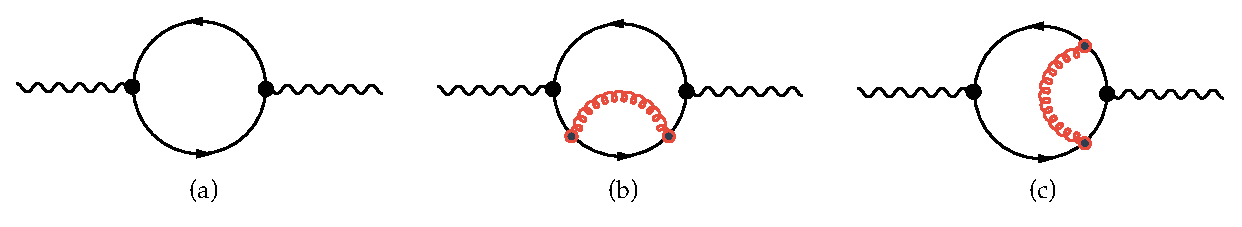
\includegraphics[width=\textwidth]{./images/correlatorLoopDiagrams.eps}
\end{figure}
E.g. we can compare the zero-loop result of the correlator \cite{Jamin2006}
\begin{equation}
  \left. \Pi^B_{\mu\nu}(q^2) \right\rvert^{1-loop} = \frac{N_c}{12\pi^2} \left( \frac{1}{\hat \epsilon} - \log\frac{(-q^2 - i0)}{\mu^2} + \frac{5}{3} + \mathcal{O}(\epsilon) \right)
\end{equation}
with \cref{eq:correlatorExpansion} and extract the first two coefficients 
\begin{equation}
  c_{00} = - \frac{5}{3} \qquad \text{and} \qquad c_{01} = 1,
\end{equation}
where $\Pi^B_{\mu\nu}(q^2)$ is not renormalized\footnote{The term $1/ \hat
  \epsilon$, which is of order 0 in $\alpha_s$, will be cancelled by renormalization.}

The second loop can also be calculated by diagram techniques resulting in \cite{Boito2011}
\begin{equation}
  \left. \Pi_V^{(1+0)}(s) \right\rvert^{2-loop} = -\frac{N_c}{12\pi^2} a_\mu \log(\frac{-s}{\mu^2}) + \cdots
\end{equation}
yielding  $c_{11} = 1$.

Beginning from three loop diagrams the algebra becomes exausting and one has to
use dedicated algorithms to compute the heigher loops. The third loop
calculations have been done in the late seventies by
\cite{Chetyrkin1979,Dine1979,Celmaster1979}. The four loop evaluation have been
completed a little more than ten years later by
\cite{Gorishnii1990,Surguladze1990}. The heighest loop published, that amounts
to $\alpha_s^4$, was published in 2008 \cite{Baikov2008} almost 20 years later.

Fixing the number of colors to $N_c=3$ the missing coefficients up to order four
in $\alpha_s$ read:
\begin{equation}
  \label{eq:adlerCoefficients}
  \begin{split}
    c_{2,1} &= \frac{365}{24} - 11 \zeta_3 - \left( \frac{11}{12} - \frac{2}{3}\zeta_3 \right) N_f \\ 
    c_{3,1} &= \frac{87029}{288} - \frac{1103}{4} \zeta_3 + \frac{275}{6}\zeta_5 \\
           &- \left( \frac{7847}{216} - \frac{262}{9} \zeta_3 + \frac{25}{9} \zeta_5 \right) N_f + \left( \frac{151}{162} - \frac{19}{27}\zeta_3\right)N_f^2 \\
   c_{4,1} &= \frac{78631453}{20736} - \frac{1704247}{432}\zeta_3 + \frac{4185}{8}\zeta_3^2 + \frac{34165}{96}\zeta_5 - \frac{1995}{16}\zeta_7,
  \end{split}
\end{equation}
where used the flavour number $N_f=3$ for the last line.

The 6-loop calculation has until today not been achieved, but Beneke und Jamin
\cite{Beneke2008} used and educated guess to estimate the coefficient
\begin{equation}
  c_{5,1} \approx 283 \pm 283.
\end{equation}

Until now we have given the coefficients $c_{n,k}$ with solely $k=1$. This
is due to the RGE, which relates coefficients with $k$ different than one to the
coefficients mentioned above. To make use of the RGE the correlator $\Pi_V^{T+L}(s)$ needs to
be a physical quantity, which can be achieved by rewriting it in terms of the
Adler function (see. \cref{eq:adlerFunction}) to:
\begin{equation}
  D_V^{(T+L)} = - s \od{\Pi_V^{(T+L)}(s)}{s} = \frac{N_c}{12 \pi^2} \sum_{n=0}^\infty a_\mu^n \sum_{k=1}^{n+1} k c_{n,k} L^{k-1},
\end{equation}
where we used $\dif L^k/ \dif s=k\ln(-s/\mu^2)^{k-1}(-1/\mu^2)$. The
Adler-function is physical quantity and has to fulfill the RGE \cref{eq:RGE}:
\begin{equation}
  -\mu \od{}{\mu} D_V^{(T+L)} = -\mu \od{}{\mu} \left( \pd{}{L} \dif L + \pd{}{a_s} \dif a_s \right) D_V^{T+L}
  = \left( 2\pd{}{L} + \beta \pd{}{a_s} \right) D_V^{T+L} = 0,
\end{equation}
where we defined the $\beta$-function in \cref{eq:betaFunction} and used $\dif L
/ \dif \mu = - 2/ \mu$. The RGE puts constraints on the $c_{n, k}$-coefficients
for different $k$s, which are not not independent anymore.

For example writing out the sum of the adler function to the second order in
$\alpha_s$ yields
\begin{equation}
  \label{eq:adlerSndOrder}
  D(s) = \frac{N_c}{12 \pi^2} \left[ c_{01} + a_\mu(c_{11} + 2 c_{12} L) + a_\mu^2(c_{21} + 2 c_{22} L + 3 c_{23} L^2) \right].
\end{equation}
Then inserting \cref{eq:adlerSndOrder} into the RGE
\begin{equation}
  4 a_\mu c_{12} + 2 a_\mu^2(2 c_{22} + 6 c_{23} L) + \beta_1 a_\mu^2(c_{11} + 2 c_{12}L) + \mathcal{O}(a_\mu^3) = 0
\end{equation}
lets us compare the coefficients order by order in $\alpha_s$. At order
$\alpha_\mu$ only the $c_{12}$ term is present and has to be zero consequently.
For $\mathcal{O}(a_\mu^2 L)$ the only $c_{23}$ exists ($c_{12}=0$) and has to
vanish as well. Finally at $\mathcal{O}(a)$ we can relate $c_{22}$ with $c_{11}$
resulting in:
\begin{equation}
  c_{12} = 0, \quad c_{22} = \frac{\beta_1 c_{11}}{4} \quad \text{and} \quad c_{23} = 0.
\end{equation}
or $D(s)$ to the first order in $\alpha_s$. Implementing the newly obtained
Adler-coefficients we can write out the adler function to the first order:
\begin{equation}
  D(s) = \frac{N_c}{12 \pi^2} \left[ c_{01} + c_{11} a_\mu \left( c_{21} - \frac{1}{2} \beta_1 c_{11} L  \right) a_\mu^2 \right] + \mathcal{O}(a_\mu^3).
\end{equation}

We have used the RGE to relate Adler-function coefficients and thus reduce its
numbers. But as we will see in the following section the RGE gives us two
different choices in the order of the computation of the perturbative
contribution to the inclusive $\tau$-decay ratio.

\subsection{Renormalisation group summation}
By making use of the RGE we have to decide about the order of mathematical
operations we perform. As the perturbative contribution $\delta^{(0)}$ is
independent on the scale $\mu$ we are confronted with two choices
\textbf{fixed-order perturbation theory} (FOPT) or \textbf{contour-improved
  perturbation theory}. Each of them yields a different result and is the main
source of error in extracting the strong coupling from $\tau$-decays.

We can write the perturbative contribution $\delta^{(0)}$ to $R_\tau$ (see
\cref{eq:rTauContributions}) in the chiral limit, such that $D^{(L)}$ vanishes as
\begin{equation}
  \label{eq:rTauDelta0}
  \delta^{(0)} = \sum_{n=1}^{\infty} a_\mu^n \sum_{k=1}^n k c_{n,k} \frac{1}{2 \pi i} \oint_{\abs{x}=1} \frac{\dif x}{x} (1-x)^3(1+x) \log \left( \frac{-M_\tau^2 x}{\mu^2} \right)^{k-1},
\end{equation}
where we inserted the expansion of $D_V^{(T+L)}$ \cref{eq:adlerFunction} into
$R_\tau$ \cref{eq:rTauFinal}. Keep in mind that the contributions from the
vector and axialvector correlator are identical in the massless case:
\begin{equation}
  D^{(T+L)} = D^{(T+L)}_V + D^{(T+L)}_A = 2 D^{(T+L)}_V.
\end{equation}

In the following we will explain both the descriptions, starting by FOPT. By
using the FOPT prescription we fix $\mu^2=m_\tau^2$ leading to
\begin{equation}
  \delta_{FO}^{(0)} = \sum_{n=1}^\infty a(m_\tau^2)^n \sum_{k=1}^n k c_{n,k} J_{k-1}
\end{equation}
where the contour integrals $J_l$ are defined by
\begin{equation}
  J_l \equiv \frac{1}{2\pi i} \oint_{\abs{x}=1} \frac{\dif x}{x} (1-x)^3(1+x) \log^l(-x).
\end{equation}
The integrals $J_l$ up to order $\alpha_s^4$ are given by \cite{Beneke2008}:
\begin{equation}
  J_0 = 1, \quad J_1 = -\frac{19}{12} \quad J_2 = \frac{265}{72} - \frac{1}{3} \pi^2, \quad J_3 = - \frac{3355}{288} + \frac{19}{12}\pi^2.
\end{equation}
Using FOPT the strong coupling $a(\mu)$, which runs with the scale $\mu$, is
fixed at $a(m_\tau^2)$ and can be taken out of the closed-contour integral. Thus
we solely to integrate over the logarithms $\log(-s/m_\tau^2)$.  

Using CIPT we can sum the logarithms by setting the scale to
$\mu^2 = -m_\tau^2 x$ in \cref{eq:rTauDelta0}, resulting in:
\begin{equation}
  \delta^{(0)}_{CI} = \sum_{n=1}^\infty c_{n,1} J_n^a(m_\tau^2),
\end{equation}
where the contour integrals $J_l$ are defined by
\begin{equation}
  J_n^a(m_\tau^2) \equiv \frac{1}{2 \pi i} \oint_{\abs{x}=1} \frac{\dif x}{x} (1-x)^3(1+x) a^n(-m_\tau^2 x).
\end{equation}
All logarithms vanish except the ones for $k=1$:
\begin{equation}
  \log(1)^{k-1} =  \begin{cases} \mbox{1} & \mbox{if } k=1, \\ \mbox{0} & k\neq 1 \end{cases}
\end{equation}
which selectes adler function coefficients $c_{n,1}$ with a fixed $k=1$. Handling the
logarithms left us with the integration of $\alpha_s(- m_\tau^2 x)$ over the closed-contour $\oint_{\abs{x}=1}$, which now
depends on the integration variable x. In general we have to decide if we want
to perform a contour integration with a constant coupling constant and variable
logarithms (FOPT) or ``constant logarithms'' and a running coupling (CIPT).

To emphasize the differences in both approaches we can calculate the
perturbative contribution $\delta^{(0)}$ to $R_\tau$ for the two different
prescriptions yielding \cite{Beneke2008}
\begin{align}
  & \quad\qquad \alpha_s^2 \qquad \alpha_s^2 \qquad \alpha_s^3 \qquad \alpha_s^4 \quad\qquad \alpha_s^5 \nonumber\\
  \delta_{FO}^{(0)} &= 0.1082 + 0.0609 + 0.0334 + 0.0174 (+ 0.0088) = 0.2200 (0.2288) \\
  \delta_{CI}^{(0)} &= 0.1479 + 0.0297 + 0.0122 + 0.0086 (+ 0.0038) = 0.1984 (0.2021).
\end{align}
The series indicate, that CIPT converges faster and that both series aproach a
different value. This discrepancy represents currently the biggest theoretical
uncertainity while extracting the strong coupling $\alpha_s$.

As today we do not know if FOPT or CIPT is the correct approach of
measuring $\alpha_s$. Therefore there are currently three ways of stating
results:
\begin{itemize}
  \item Quoting the average of both results.
  \item Quoting the CIPT result.
  \item Quoting the FOPT result.
\end{itemize}

We follow the approach of Beneke and Jamin \cite{Benke2008} who have shown
advantages of FOPT over CIPT.


\section{Non-Perturbative OPE Contribution}
The perturbative contribution to the Sum-Rule, that we have seen so far, is the
dominant one. With
\begin{equation}
  \begin{split}
    R_\tau^{FOPT} &= \\ 
    R_\tau^{CIPT} &=  
  \end{split}
\end{equation}

The NP vs perturbative contributions can be varied by choosen different weights
than $\omega_\tau$.


\subsection{Dimension four}
For the OPE contributions of dimension four we have to take into account the
terms with masses to the fourth power $m^4$, the quark condensate multiplied by
a mass $m \langle \anti{q} q \rangle$ and the glucon condensate $\langle GG
\rangle$. The resulting expression can be taken from the appendix of
\cite{Pich1999}, yielding:
\begin{equation}
  \left. D_{ij}^{(L+T)}(s) \right\rvert_{D=4} = \frac{1}{s^2} \sum_n \Omega^{(1+0)}(s/\mu^2)a^n,
\end{equation}
where
\begin{equation}
  \begin{split}
    \Omega_n^{(1+0)} (s/\mu^2) &\,=\, \frac{1}{6}\langle aGG \rangle p_n^{(L+T)}(s/\mu^2) + \sum_k m_k \langle \anti{q}_k q_k \rangle r_n^{(L+T)}(s/\mu^2) \\
    &\,+ 2\langle m_i \anti{q}_i q_i + m_j \anti{q}_j q_j \rangle q_n^{(L+T)} (s/\mu^2) \pm \frac{8}{3} \langle m_j \anti{q}_i q_i + m_i \anti{q}_j q_j \rangle t_n^{(L+T)} \\
    &\,- \frac{3}{\pi^2} (m_i^4 + m_j^4) h_n^{(L+T)} (s/\mu^2) \mp \frac{5}{\pi^2} m_i m_j (m_i^2 + m_j^2) k_n^{(L+T)}(s/\mu^2)\\
    &\,+ \frac{3}{\pi^2} m_i^2 m_j^2 g_n^{(L+T)}(s/\mu^2) + \sum_k m_k^4 j_n^{(L+T)}(s/\mu^2) + 2 \sum_{k \neq l} m_k^2 m_l^2 u_n^{(L+T)}(s/\mu^2)
  \end{split}
\end{equation}
The perturbative expansion coefficients are known to $\mathcal{O}(a^2)$ for the
condensate contributions,
\begin{equation}
  \begin{array}{lll}
    p_0^{(L+T)}=0, & p_1^{(L+T)}=1, & p_2^{(L+T)}=\frac{7}{6}, \\
    r_0^{(L+T)}=0, & r_1^{(L+T)}=0, & r_2^{(L+T)}=-\frac{5}{3}+\frac{8}{3}\zeta_3-\frac{2}{3}\log(s/\mu^2), \\
    q_0^{(L+T)}=1, & q_1^{(L+T)}=-1, & q_2^{(L+T)}=-\frac{131}{24}+\frac{9}{4}\log(s/\mu^2) \\
    t_0^{(L+T)}=0 & t_1^{(L+T)}=1, & t_2^{(L+T)}=\frac{17}{2}+\frac{9}{2}\log(s/\mu^2).
  \end{array}
\end{equation}
while the $m^4$ terms have been only computed to $\mathcal{O}(a)$
\begin{equation}
  \begin{array}{lll}
    h_0^{(L+T)}=1-1/2 \log(s/\mu^2), & h_1^{(L+T)}=\frac{25}{4}-2\zeta_3-\frac{25}{6}\log(s/\mu^2)-2 \log(s/\mu^2)^2, \\
    k_0^{(L+T)}=0, & k_1^{(L+T)}=1-\frac{2}{5}\log(s/\mu^2), \\
    g_0^{(L+T)}=1, & g_1^{(L+T)}=\frac{94}{9}-\frac{4}{3}\zeta_3-4 \log(s/\mu^2), \\
    j_0^{(L+T)}=0, & j_1^{(L+T)}=0, \\
    u_0^{(L+T)}=0, & u_2^{(L+T)}=0.
  \end{array}
\end{equation}

\subsection{Dimension six and eight}
Our application of dimension six contributions is founded in \cite{Braaten1991}
and has previously been calculated beyond leading order by \cite{Lanin1986}.
The operators appearing are the masses to the power six $m^6$, the four-quark
condensates $\langle \anti q q \anti q q \rangle$, the three-gluon condensates
$\langle g^3 G^3 \rangle$ and lower dimensional condensates multiplies by the
corresponding masses, such that in total the mass dimension of the operator will
be six.
As there are too many parameters to be fitted with experimental data we have to
omit some of them, starting with the three-gluon condensate, which does not
contribute at leading order. The four-quark condensates known up to
$\mathcal{O}(a^2)$, but we will make use of the \textit{vacuum saturation
  approach} \cite{Beneke2008,Braaten1991,Shifman1978} to express them in quark, anti-quark condensates $\langle q \anti{q} \rangle$.
In our work we take the simplest approach possible: Introducing an effective
dimension six coefficient $\rho_{V/A}^{(6)}$ divided by the appropiate power in s
\begin{equation}
  \left. D_{ij,V/A}^{(1+0)} \right\rvert_{D=6} = 0.03 \frac{\rho_{V/A}^{(6)}}{s^3}
\end{equation}

As for the dimension eigth contribution the situation is not better than the
dimension six one we keep the simplest approach, leading to
\begin{equation}
  \left. D_{ij,V/A}^{(1+0)} \right\rvert_{D=8} = 0.04 \frac{\rho_{V/A}^{(8)}}{s^4}.
\end{equation}


\subsection{Duality Violations}


\section{Experiment}
The $\tau$-decay data we use to perform our QCD-analysis is from the
\textbf{ALEPH} experiment. The ALEPH experiment was located at the
large-electron-positron (LEP) collider at CERN laboratory in Geneva. LEP started
producing particles in 1989 and was replaced in the late 90s by the
large-hadron-collider, which makes use of the same tunnel of 27km circumference.
The data produced within the experiment is still maintained by former ALEPH
group members under led by M. Davier, which have performed regular updates on
the data-sets \cite{Davier2013,Davier2008,Schael2005}.

The measured spectral functions for the Aleph data are defined in
\cite{Davier2007} and given for the transversal and longitudinal components separatly:
\begin{equation}
  \begin{split}
    \rho^{(T)}_{V/A}(s) &= \frac{m_\tau^2}{12 \abs{V_{ud}^2}S_{EW}} \frac{\mathcal{B}(\tau^- \to V^-/A^- \nu_\tau)}{\mathcal{B}(\tau^- \to e^- \anti{\nu}_e \nu_\tau)} \\
    &\quad\times \frac{\dif N_{V/A}}{N_{V/A}\dif s} \left[ \left( 1 - \frac{s}{m_\tau^2} \right)^2 \left( 1 + \frac{2s}{m_\tau^2} \right) \right]^{-1} \\
  \rho^{(L)}_{A}(s) &= \frac{m_\tau^2}{12 \abs{V_{ud}^2 S_{EW}}} \frac{\mathcal{B}(\tau^- \to \pi^-(K^-) \nu_\tau)}{\mathcal{B}(\tau^- \to e^- \anti{\nu}_e \nu_\tau)} \times \frac{\dif N_A}{N_A \dif s} \left( 1 - \frac{s}{m_\tau^2} \right)^{-2}.
  \end{split}
\end{equation}

\begin{equation}
  \mathcal{B}_e = ...
\end{equation}

\begin{equation}
  R_{\tau, V/A} = \frac{B_{V/A, \tau}}{B_e}
\end{equation}

The data relies on a separation into vector and axial-vector channels. In the
case of the Pions this can be achieved via counting. The vector channel is
characterized by a negative parity, whereas the axial-vector channel has
positive parity. A quark has by definition positive parity, thus an anti-quark
has a negative parity. A meson, like the Pion particle, is a composite particle
consiting of an quark an anti-quark. Consequently a single Pion carries negative
parity, an even number of Pions carries positive parity and an odd number of
Pions carries negative parity:
\begin{equation}
  n \times \pi = \begin{cases} \mbox{vector} & \mbox{if } n \text{ is even}, \\ \mbox{axial-vector} & \mbox{otherwise} \end{cases}.
\end{equation}

The contributions to the vector and axial channel can be seen in
\textcolor{red}{figure}. The dominant modes in the vector case are
\cite{Davier2006} $\tau^- \to \pi^-\pi^0 \nu_\tau$ and the $\tau^- \to \pi^-
\pi^- \pi^+ \pi^0 \nu_\tau$. The first of these is produced by the $\rho(770)$
meson, which in contrary to the pions carries angular momentum of one, which is
also clearly visible as peak around $\SI{770}{\giga\eV}$ in
\textcolor{red}{figure vector}. The dominant modes in the axial-vector case are
$\tau^-\to \pi^-\nu_\tau$, $\tau^-\to \pi^- \pi^0 \pi^0 \nu_\tau$ and
$\tau^- \to \pi^- \pi^- \pi^+\nu_\tau$. Here the three pion final states stem
from the $a_1^-$-meson, which is also clearly visible as a peak in \textcolor{red}{figure}.
\begin{figure}
    \centering
    \begin{subfigure}[b]{0.49\textwidth}
        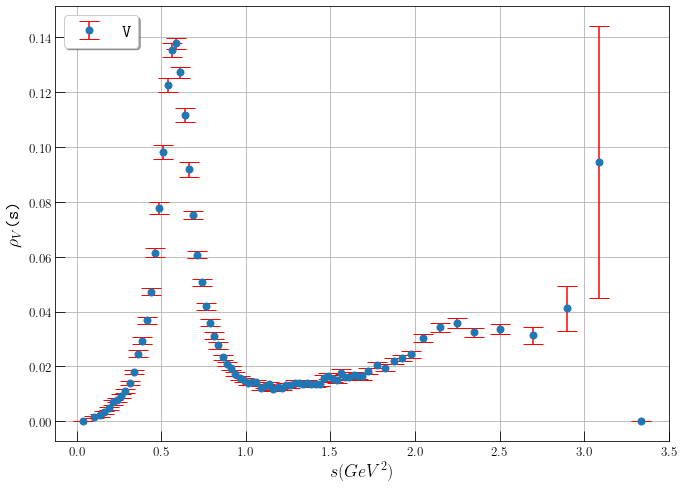
\includegraphics[width=\textwidth]{./images/specFuncAleph_V.png}
        \caption{A gull}
        \label{fig:gull}
    \end{subfigure}
    \begin{subfigure}[b]{0.49\textwidth}
        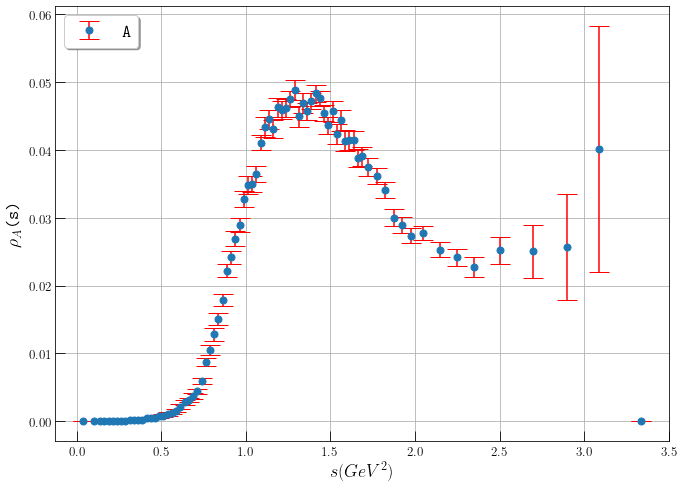
\includegraphics[width=\textwidth]{./images/specFuncAleph_A.png}
        \caption{A mouse}
        \label{fig:mouse}
    \end{subfigure}
    \begin{subfigure}[b]{0.8\textwidth}
      \centering
      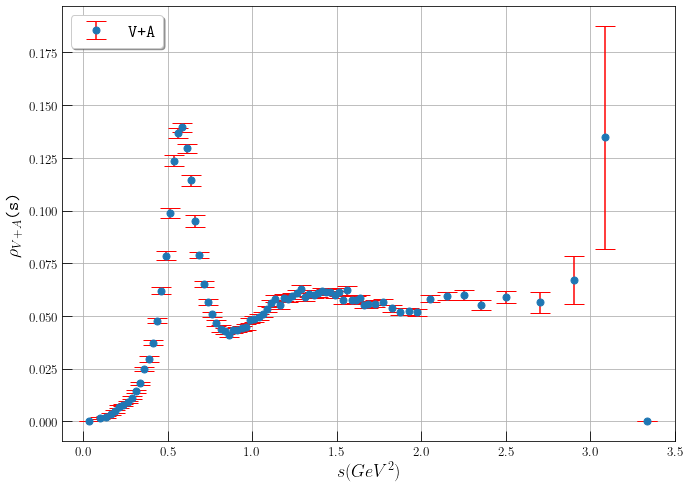
\includegraphics[width=\textwidth]{./images/specFuncAleph_VpA.png}
      \label{fig:}
    \end{subfigure}
    \caption{Pictures of animals}\label{fig:animals}
\end{figure}

wavy => DV
OPE cannot reproduce
suppressed in VpA
regions below 1.5 GeV can still not be applied

The different inclusive $\tau$-decay ratios are then given by
\begin{align}
  R_{\tau,V} &= ...
\end{align}



\end{document}